\documentclass[10pt]{article}



%вставка изображений и картинок всяких

\usepackage{graphicx}
\newcommand{\incfig}[1]{%
    \def\svgscale{1.5}
    \import{./figures/}{#1.pdf_tex}
}
\graphicspath{{pictures/}}
\DeclareGraphicsExtensions{.pdf,.png,.jpg, .jpeg, .tex}

\usepackage{booktabs} % для таблиц
\usepackage{enumitem} % для списков


% Шрифты

\usepackage[english,russian]{babel}
\usepackage[T1]{fontenc}
\usepackage{libertine}


\usepackage{titling} % для \maketitle
\usepackage{textcomp}% специальные символы в тексте

\usepackage{mathtext}
\usepackage{amsmath,amsfonts,amssymb,amsthm,mathtools} % математика
\usepackage{icomma} % умная запятая
\usepackage{import} %  импортирование


\usepackage{pdfpages} % мультри-пдф страницы
\usepackage{transparent} % что-то про цвета


\usepackage{caption} % комментарии к figure
\usepackage{epigraph} % эпиграфы

\usepackage{comment} % удобные комментарии
\usepackage{xfrac} % дроби
\usepackage{moresize} % все размеры шрифтов
\usepackage{dsfont} % mathbb для всего


% Окружения для математики:

\newtheorem{statement}{Предложение}
\newtheorem{corollary}{Следствие}
\newtheorem{theorem}{Теорема}
\theoremstyle{definition}
\newtheorem{definition}{Определение}


\newtheorem{example}{Пример}
\newtheorem{homework}{Домашнее задание}
\newtheorem{antiexample}{Антиример}
\newtheorem{lemma}{Лемма}
\theoremstyle{remark}
\newtheorem*{remark}{Замечание}
\newtheorem*{exercise}{Упражнение}

% Настройки счетчиков:

%\numberwithin{equation}{section} % Number equations within sections (i.e. 1.1, 1.2, 2.1, 2.2 instead of 1, 2, 3, 4)
%\numberwithin{figure}{section} % Number figures within sections (i.e. 1.1, 1.2, 2.1, 2.2 instead of 1, 2, 3, 4)
%\numberwithin{table}{section} % Number tables within sections (i.e. 1.1, 1.2, 2.1, 2.2 instead of 1, 2, 3, 4)

% Геометрия файла:

\usepackage{geometry}

\setlist{noitemsep} % No spacing between list items

\geometry{left=1.5cm,right=1.5cm,top=2.5cm,bottom=2cm, a4paper}

% Счётчики разделов:


%\sectionfont{\vspace{6pt}\centering\normalfont\scshape} % \section{} styling
%\subsectionfont{\normalfont\bfseries} % \subsection{} styling
%\subsubsectionfont{\normalfont\itshape} % \subsubsection{} styling
%\paragraphfont{\normalfont\scshape} % \paragraph{} styling

\newcommand{\RNumb}[1]{\uppercase\expandafter{\romannumeral #1\relax}}

\renewcommand\thesection{\arabic{section}.}
\renewcommand\thesubsection{\thesection\arabic{subsection}}
\renewcommand\thesubsubsection{\RNumb{\arabic{subsubsection}}}
\renewcommand{\bf}{\textbf}

% Колонтитулы

\usepackage{fancyhdr}
\pagestyle{fancy}
\fancyhf{} % clear all fields
\fancyhead[L]{\rightmark}
\fancyhead[R]{\thepage}

\renewcommand{\sectionmark}[1]{%
  \markright{\thesection\ #1}}%
\setlength{\headheight}{17.0pt}
\addtolength{\topmargin}{-2.49998pt}



% Операторы:

\DeclareMathOperator{\ord}{ord}
\DeclareMathOperator{\ld}{ld}
\DeclareMathOperator{\id}{id}
\DeclareMathOperator{\exi}{exi}
\DeclareMathOperator{\osc}{osc}
\DeclareMathOperator{\num}{num}
\DeclareMathOperator{\Char}{char}
\DeclareMathOperator{\card}{Card}
\DeclareMathOperator{\sk}{sk}
\DeclareMathOperator{\den}{den}
\DeclareMathOperator{\essup}{essup}
\DeclareMathOperator{\ran}{ran}
\DeclareMathOperator{\rank}{rank}
\DeclareMathOperator{\dom}{dom}
\DeclareMathOperator{\diam}{diam}
\DeclareMathOperator{\dist}{dist}
\DeclareMathOperator{\disc}{disc}
\DeclareMathOperator{\rad}{rad}
\DeclareMathOperator{\supp}{supp}

\DeclareMathOperator{\sign}{sign}
\DeclareMathOperator{\Int}{Int}
\DeclareMathOperator{\RelInt}{RelInt}
\DeclareMathOperator{\Cl}{Cl}
\DeclareMathOperator{\Class}{\mathcal{C}\mathbf{\ell}}
\DeclareMathOperator{\CW}{CW}
\DeclareMathOperator{\Ideals}{Ideals}
\DeclareMathOperator{\pr}{pr}
\DeclareMathOperator{\ind}{ind}
\DeclareMathOperator{\Af}{Aff}
\DeclareMathOperator{\Aut}{Aut}
\renewcommand{\Im}{\mathop{\mathrm{Im}}\nolimits}
\DeclareMathOperator{\Conv}{conv}
\DeclareMathOperator{\Fr}{Fr}
\DeclareMathOperator{\Tr}{Tr}
\DeclareMathOperator{\Nm}{\mathrm{N}}
\DeclareMathOperator{\Span}{span}
\DeclareMathOperator{\Map}{Map}
\DeclareMathOperator{\Hom}{Hom}
\DeclareMathOperator{\Ker}{Ker}
\DeclareMathOperator{\Ext}{Ext}
\DeclareMathOperator{\Div}{Div}
\DeclareMathOperator{\NRad}{NRad}
\DeclareMathOperator{\Coker}{Coker}
\DeclareMathOperator{\Gal}{Gal}
\DeclareMathOperator{\Specm}{Specm}
\DeclareMathOperator{\Spec}{Spec}
\DeclareMathOperator{\Ht}{ht}
\DeclareMathOperator{\End}{End}
\DeclareMathOperator{\Rad}{Rad}
\DeclareMathOperator{\Ann}{Ann}
\DeclareMathOperator{\Vol}{Vol}
\DeclareMathOperator{\res}{res}
\DeclareMathOperator{\Gr}{Gr}
\DeclareMathOperator{\Bl}{Bl}
\DeclareMathOperator{\mult}{mult}
\DeclareMathOperator{\cont}{cont}
\DeclareMathOperator{\area}{area}

\renewcommand{\Re}{\mathop{\mathrm{Re}}\nolimits}
\DeclarePairedDelimiter\lr{(}{)}
\DeclareRobustCommand{\divby}{%
     \mathrel{\text{\vbox{\baselineskip.65ex\lineskiplimit0pt\hbox{.}\hbox{.}\hbox{.}}}}%
}
\newcommand{\eqdef}{\stackrel{\mathrm{def}}{=}}
\DeclareRobustCommand{\notdivby}{%
     \!\!\not\;\divby%
}
\newcommand{\lei}{\trianglelefteq}

%%%% гиперссылки
\usepackage{xcolor} % цвета
\usepackage[unicode, pdftex]{hyperref}
\hypersetup{%
  colorlinks=false,
  linkbordercolor=cyan
}

% Буковы

\newcommand{\N}{\mathbb{N}}			 		
\newcommand{\Z}{\mathbb{Z}}			
\newcommand{\Q}{\mathbb{Q}}		
\newcommand{\R}{\mathbb{R}}	
\let\oldC\C
\renewcommand{\C}{\mathbb{C}} 				
\newcommand{\F}{\mathbb{F}}	
 
\let\oldAA\AA
\renewcommand{\AA}{\mathbb{A}}				
\newcommand{\DD}{\mathbb{D}}  						
\newcommand{\EE}{\mathbb{E}} 			
\newcommand{\HH}{\mathbb{H}}					
\newcommand{\KK}{\mathbb{K}} 					
\newcommand{\OO}{\mathbb{O}} 		
\newcommand{\PP}{\mathbb{P}}			
\let\oldSS\SS		
\renewcommand{\SS}{\mathbb{S}}						
\newcommand{\TT}{\mathbb{T}} 			

\newcommand{\cA}{\mathcal{A}}
\newcommand{\cB}{\mathcal{B}}
\newcommand{\cC}{\mathcal{C}}
\newcommand{\cD}{\mathcal{D}}
\newcommand{\cE}{\mathcal{E}}
\newcommand{\cF}{\mathcal{F}}
\newcommand{\cG}{\mathcal{G}}
\newcommand{\cH}{\mathcal{H}}
\newcommand{\cI}{\mathcal{I}}
\newcommand{\cJ}{\mathcal{J}}
\newcommand{\cK}{\mathcal{K}}
\newcommand{\cL}{\mathcal{L}}
\newcommand{\cM}{\mathcal{M}}
\newcommand{\cN}{\mathcal{N}}
\newcommand{\cO}{\mathcal{O}}
\newcommand{\cQ}{\mathcal{Q}}
\newcommand{\cP}{\mathcal{P}}
\newcommand{\cR}{\mathcal{R}}
\newcommand{\cS}{\mathcal{S}}
\newcommand{\cT}{\mathcal{T}}
\newcommand{\cU}{\mathcal{U}}
\newcommand{\cV}{\mathcal{V}}
\newcommand{\cW}{\mathcal{W}}
\newcommand{\cX}{\mathcal{X}}
\newcommand{\cY}{\mathcal{Y}}
\newcommand{\cZ}{\mathcal{Z}}
			
\newcommand{\rD}{\mathrm{D}}
\newcommand{\rK}{\mathrm{K}}			
\newcommand{\rP}{\mathrm{P}}
\newcommand{\rT}{\mathrm{T}}			

\newcommand{\fA}{\mathfrak{A}}
\newcommand{\fQ}{\mathfrak{Q}}
\newcommand{\fB}{\mathfrak{B}}
\newcommand{\fT}{\mathfrak{T}}
\newcommand{\fK}{\mathfrak{K}}
\newcommand{\fM}{\mathfrak{M}}
\newcommand{\fL}{\mathfrak{L}}
\newcommand{\fR}{\mathfrak{R}}
\newcommand{\fP}{\mathfrak{P}}
\newcommand{\fC}{\mathfrak{C}}
\newcommand{\fX}{\mathfrak{X}}
\newcommand{\fS}{\mathfrak{S}}

\newcommand{\fm}{\mathfrak{m}}
\newcommand{\fb}{\mathfrak{b}}
\newcommand{\ff}{\mathfrak{f}}
\newcommand{\fp}{\mathfrak{p}}
\newcommand{\fq}{\mathfrak{q}}
\newcommand{\fh}{\mathfrak{h}}
\newcommand{\fo}{\mathfrak{o}}
\newcommand{\fe}{\mathfrak{e}}
\newcommand{\ft}{\mathfrak{t}}
\newcommand{\fr}{\mathfrak{r}}
\newcommand{\fg}{\mathfrak{g}}
\newcommand{\fl}{\mathfrak{l}}
\newcommand{\fa}{\mathfrak{a}}
\newcommand{\fd}{\mathfrak{d}}
\newcommand{\qAff}{\mathsf{qAff}}
\newcommand{\Aff}{\mathsf{Aff}}
\newcommand{\Alg}{\mathsf{Alg}}
\newcommand{\Set}{\mathsf{Set}}
\newcommand{\Mod}{\mathsf{Mod}}
\usepackage{esint}
\renewcommand{\v}{\upsilon}
\newcommand{\vp}{\v_{p}}

% Tikz и графика:


\usepackage{pgfplots}
\usepackage{tikz}
\usetikzlibrary{3d,perspective}
\usetikzlibrary{animations}
\usetikzlibrary{cd}
\usepackage{mathtools}
\pgfplotsset{width=6cm,compat=newest}

\newcommand{\RNum}[1]{\uppercase\expandafter{\romannumeral #1\relax}}




\usepackage{multicol}
\usepackage{pdflscape}
\usepackage{wrapfig}
\begin{document}
	\begin{landscape}

	\pagestyle{empty}
	\begin{multicols}{2}

	\centerline{\bf{Серия 1. Групповая практика. }}

	\epigraph{Symmetry is a vast subject, significant in art and nature. Mathematics lies at its root, and it would be hard to find a better one on which to demonstrate the working of the mathematical intellect.}{Герман Вейль}

	\bf{0.} Докажите, что композиция отображений ассоциативна, т.е., что для $f \colon X \to Y, g \colon Y \to Z, \ h \colon Z \to T$
	\[
		h \circ (g \circ f) = (h \circ g) \circ f.
	\]

	\bf{1.} а) Докажите, что нейтральный элемент группы единственнен. б) Докажите, что для любого элемента $g \in G$ существует единственный обратный элемент $g^{-1}$. 

	\bf{2.} а) Опишите (словами и геометрически) группу симметрий квадрата. б) Найдите в ней такой элемент $x$, что $x^3 = R_{90^{\circ}}$. в) Найдите три симметрии квадрата $f, g, h \in D_{4}$, для которых $fg = gh$, но $f \neq h$.

	\begin{definition} 
		\emph{Полугруппой} называют множество с ассоциативной бинарной операцией. 
	\end{definition}

	\bf{3.} а)  Пусть в группе $G$ для любого $g \in G$ выполнено $g^2 = e$. Докажите, что $G$~--- абелева группа.  б) Пусть $G$~--- конечная полугруппа. Докажите, что существует такой элемент $g \in G$, что $g^2 = g$.

	\bf{4.} Карлсон, убежавший от бабушки, сидит на дереве с одним носком, надетым на одну из ног. Он может оставить носок на ноге, переодеть его на другую ногу или вывернуть его, оставив на той же ноге. Опишите группу, которая получается из таких преобразованиях. 

	\bf{5.} а) Опишите группу симметрий прямоугольника, который не является квадратом. б) Опишите группу симметрий параллелипипеда, который не является кубом (например, спичечного коробка). в) Обобщите предыдущие два пункта на высшие размерности. 

	\begin{center}
	\begin{minipage}{6in}
		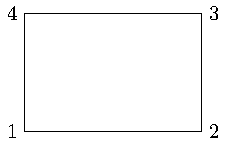
\includegraphics[width=0.25\textwidth]{pic/pic_1.pdf}
		\hspace{10mm}
		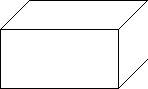
\includegraphics[width=0.25\textwidth]{pic/pic_2.pdf}
	\end{minipage}
	\end{center}


	\columnbreak

	\centerline{\bf{Серия 1. Групповая практика. }}

	\epigraph{Symmetry is a vast subject, significant in art and nature. Mathematics lies at its root, and it would be hard to find a better one on which to demonstrate the working of the mathematical intellect.}{Герман Вейль}

	\bf{0.} Докажите, что композиция отображений ассоциативна, т.е., что для $f \colon X \to Y, g \colon Y \to Z, \ h \colon Z \to T$
	\[
		h \circ (g \circ f) = (h \circ g) \circ f.
	\]

	\bf{1.} а) Докажите, что нейтральный элемент группы единственнен. б) Докажите, что для любого элемента $g \in G$ существует единственный обратный элемент $g^{-1}$. 

	\bf{2.} а) Опишите (словами и геометрически) группу симметрий квадрата. б) Найдите в ней такой элемент $x$, что $x^3 = R_{90^{\circ}}$. в) Найдите три симметрии квадрата $f, g, h \in D_{4}$, для которых $fg = gh$, но $f \neq h$.

	\begin{definition} 
		\emph{Полугруппой} называют множество с ассоциативной бинарной операцией. 
	\end{definition}

	\bf{3.} а)  Пусть в группе $G$ для любого $g \in G$ выполнено $g^2 = e$. Докажите, что $G$~--- абелева группа.  б) Пусть $G$~--- конечная полугруппа. Докажите, что существует такой элемент $g \in G$, что $g^2 = g$.

	\bf{4.} Карлсон, убежавший от бабушки, сидит на дереве с одним носком, надетым на одну из ног. Он может оставить носок на ноге, переодеть его на другую ногу или вывернуть его, оставив на той же ноге. Опишите группу, которая получается из таких преобразованиях. 

	\bf{5.} а) Опишите группу симметрий прямоугольника, который не является квадратом. б) Опишите группу симметрий параллелипипеда, который не является кубом (например, спичечного коробка). в) Обобщите предыдущие два пункта на высшие размерности. 

	\begin{center}
	\begin{minipage}{6in}
		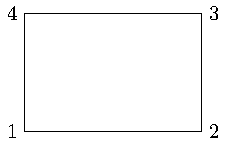
\includegraphics[width=0.25\textwidth]{pic/pic_1.pdf}
		\hspace{10mm}
		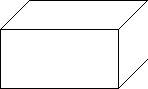
\includegraphics[width=0.25\textwidth]{pic/pic_2.pdf}
	\end{minipage}
	\end{center}


	

	\end{multicols}
	\end{landscape}


\end{document}